% !TeX root = ../main.tex
% Add the above to each chapter to make compiling the PDF easier in some editors.

\chapter{Implementation}\label{chapter:implementation}
After discussing the concept of a checkpoint management system, this chapter focuses on the actual implementation of a prototype in C++ utilising the API of Genode version 21.08. 
\section{Run-Script}
"The Genode OS Framework comes with a custom build system that is designed for the creation of highly modular and portable systems software." \cite{build_system} This build directory targets a specific platform, in our case the Fiasco.OC microkernel and the RealView PBX-A9 hardware architecture. From within these directories system scenarios are executed via their run-script, a file responsible for building the components, creating a boot directory, configuring the init process, creating a bootable system image, and finally executing the system image. \cite{build_system}
This script is essential to the system scenario executed, and therefore important aspects and how they were implemented, are presented.
\subsection{Package Management}
The advantages of the run tool are automation of building, configuration, integration and testing. This results in one image with a certain set of features. If any part of the automated chain changes, a completely new image has to be created, which means having to recompile all components during the process of building. For complicated system scenarios with many components, this induces an unnecessary overhead. The concept of depots aims to resolve this issue: archives are downloaded preemptively and then imported by the run script. \cite{package_management} The following listing shows the code used for the building part of the \verb|manager.run| script, which executes the system scenario of the checkpoint management system.

\begin{lstlisting}[caption={Importing of depot archives and subsequent building in manager.run.}]
import_from_depot [depot_user]/src/[base_src] \
                  [depot_user]/pkg/[drivers_nic_pkg] \
                  [depot_user]/src/nic_router \
                  [depot_user]/src/init \
                  [depot_user]/src/libc \
                  [depot_user]/src/vfs_lwip \
                  [depot_user]/src/vfs \
                  [depot_user]/src/stdcxx

build { manager rtcr_dummy nas}
\end{lstlisting}
\verb|[depot_user]| stands for the origin of the archives contained within the directory, as it is possible to download an archive with an identical name to the archive of another user. \verb|[base_src]| refers to the base archives corresponding to the selected microkernel and hardware architecture. The \verb|nic_router| archive together with the NIC-drivers package is responsible for the network interface, which architecture was explained in section \ref{subsection:network}. The socket API that uses lwIP is integrated into the libc library, which depends on the virtual file system (vfs). These archives are therefore also imported. Of the two remaining archives, \verb|init| represents the initial component serving as a parent to the components making up the system scenario, while \verb|stdcxx| is a library containing the C++ standard library ported to Genode OS.

Ultimately, only the manager, rtcr\_dummy and nas components have to be compiled and built with every execution, with all components that don't change being imported as archives, significantly reducing the overhead.
\subsection{Configuration of the Init Component}
Init is the component which controls the execution of all further components making up the system scenario. The policy of init is defined by configuring it and all its children together with the services they require and provide inside an XML config in the run-script. Within the root config tags, the services provided by init's parent core, like ROM, IO\_MEM and CPU, and the concrete components of the system scenario are listed. In our case, outside of the manager, RTCR and NAS programs, this also includes the timer, drivers and nic\_router components. After presenting and explaining the configuration of the main components, their interplay through the nic\_router and its configuration, is also shown. \cite{init_config}
\subsubsection{Main Components}
The basic elements of a component configuration are its name, its RAM and capability quotas, the services it provides to other components, and a routing table to services that are being offered by others. If RAM or capability quotas are not stated explicitly, the component is configured with a default quota defined in the configuration of init. The following listing shows the manager definition, where name, quota and the provided service called "Manager", which is utilised when RTCR and manager are on the same ECU, are self-evident. In the system scenario making up the prototype, only one manager without any redundant components is employed, because integrating and testing another manager into the system was too time-intensive. The routing table can be found within the \verb|<route>| tags. Here the route to the "Nic" service is stated by pointing to the nic\_router component, whereas for all other services, a default route pointing to init's parent or any other child of init is utilised. \cite{init_config}
\begin{lstlisting}[language=XML, caption={Configuration of the manager component.}]
<start name="manager">
    <resource name="RAM" quantum="10M"/>
    <provides> <service name="Manager"/> </provides>
    <config port="1024" nas_ip="10.0.2.2" nas_port="1027" rtcr_info_port="1025" rtcr_migr_port="1026">
        <vfs>
            <dir name="dev"> <log/> </dir>
            <dir name="socket">
                    <lwip ip_addr="10.0.0.2"
                          netmask="255.255.255.0"
                          gateway="10.0.0.1"/>
            </dir>
        </vfs>
        <libc stdout="/dev/log" stderr="/dev/log" socket="/socket"/>
    </config>
    <route>
		<service name="Nic"> <child name="nic_router"/> </service>
		<any-service> <parent/> <any-child/> </any-service>
	</route>
</start>
\end{lstlisting}
The remainder is necessary information for networking and diagnostic printing. Directly within the \verb|<config>| tags, the static ports and IPs of certain services provided over Ethernet are defined. Because the configuration is provided to the components as a ROM-session, it is possible to read from these definitions from within the actual implementation and thus prevent hard coding numbers. These ports and services are:
\begin{itemize}
    \item 1024: The port through which messages to the manager's main interface are handled.
    \item 1025: The RTCR provides an interface for system information to allow the manager to decide where to migrate a checkpoint to on this port.
    \item 1026: Checkpoints sent to this port are restored under the RTCR running on the respective ECU.
    \item 1027: This port is where the NAS handles both checkpoint storage and retrieval requests.
\end{itemize}
Another important element that has to be configured is the virtual file system (VFS), as libc depends on it, and the socket API we wish to use relies on libc. In Genode, file systems are component-local. Therefore each component that uses the VFS has its own root directory, from which the file system structure is spanned. Inside the \verb|<vfs>| tags this structure can be customised with any conceivable directories or files, but in this case two conventional directories are introduced to the file system of the manager component. Firstly, the directory "dev" is added, within which the \verb|<log/>| file-system plugin adds a file called \verb|log|. This file forwards everything written to it to the Log session of the program.
Inside the second directory named "socket", the IP-stack plugin \verb|<lwip/>| configures the network stack with an IP-address, a netmask and a standard gateway.

Finally libc itself is also equipped with standard outputs and a socket interface by declaring the environment variables \verb|stdout|, \verb|stderr| and \verb|socket|, using the previously defined file system structure. \cite{vfs_basics} \cite{vfs_networking}
\newline \newline
The other main component besides the NAS, of which the configuration is very similar to that of the manager and therefore not further presented, is the RTCR. However, because it would have to be ported to the current version of Genode, a dummy is employed. The configuration of one such RTCR-dummy is shown in the following listing. For reasons of testing, the system scenario is equipped with two RTCR-dummies with different names using the same source code. This step is evident by the additional \verb|<binary>| tag, which contains the name of the source binary. Another difference is that the routing table additionally points to the service offered by the manager component.
\begin{lstlisting}[language=XML, caption={Configuration of one of the two RTCR-dummy components.}]
<start name="rtcr_dummy_1">
    <binary name="rtcr_dummy"/>
    <resource name="RAM" quantum="10M"/>
    <config name="dummy_1" ip="10.0.1.2" mac="57406533673528" manager_ip="10.0.0.2" manager_port="1024" info_port="1025" migr_port="1026">
        <vfs>
            <dir name="dev"> <log/> </dir>
            <dir name="socket"> <lwip ip_addr="10.0.1.2"
                                      netmask="255.255.255.0"
                                      gateway="10.0.1.1"/>
            </dir>
        </vfs>
        <libc stdout="/dev/log" stderr="/dev/log" socket="/socket"/>
    </config>
    <route>
		<service name="Nic"> <child name="nic_router"/> </service>
	    <service name="Manager"> <child name="manager"/> </service>
		<any-service> <parent/> <any-child/> </any-service>
	</route>
</start>
\end{lstlisting}
The config section of the RTCR-dummy is very similar to the manager, except the extra variable definitions for name, IP- and MAC-address of the component. This seemingly superfluous information is necessary, because no way was found to determine these values dynamically from the component name in the first, and from the network stack in the last two cases. The name is required for diagnostics, while IP and MAC need to be transmitted to the manager for purposes of RTCR interface access and identification, respectively. Here the MAC is saved as an 48 bit integer, which translated into conventional notation is 52:54:00:12:34:56. The IP- and MAC-addresses of the second RTCR-dummy are those of the first incremented by one.
\subsubsection{Nic\_router}
To ultimately enable the components to communicate using their respective network stacks, a mediation unit is required. This mediation unit is the NIC-router, as presented in section \ref{subsection:network}. With this unit in play, the system scenario closely resembles two applications on different ECUs connected through a real router, as is conceptualised. The configuration of the router is shown in the following listing.
\begin{lstlisting}[language=XML, caption={Configuration of the NIC-router component.}] 
<start name="nic_router" caps="1000">
    	<resource name="RAM" quantum="32M"/>
	<provides>
		<service name="Nic"/>
		<service name="Uplink"/>
	</provides>
	<config>
	    <policy label_prefix="drivers" domain="uplink"/>
		<policy label_prefix="manager" domain="manager"/>
		<policy label_prefix="rtcr_dummy" domain="rtcr"/>
		<policy label_prefix="nas" domain="nas"/>

		<domain name="uplink">
			<nat domain="manager" tcp-ports="100"/>
			<nat domain="rtcr" tcp-ports="100"/>
			<nat domain="nas" tcp-ports="100"/>
		</domain>
		<domain name="manager" interface="10.0.0.1/24">
		    <tcp dst="10.0.1.0/24">
		        <permit port="1025" domain="rtcr" />
		        <permit port="1026" domain="rtcr" />
		    </tcp>
		    <tcp dst="10.0.2.0/24">
		        <permit port="1027" domain="nas" />
		    </tcp>
		</domain>
		<domain name="rtcr" interface="10.0.1.1/24">
			<tcp dst="10.0.0.0/24">
			    <permit-any domain="manager" />
			</tcp>
		</domain>
		<domain name="nas" interface="10.0.2.1/24">
		</domain>
	</config>
</start>
\end{lstlisting}
As presented in section \ref{subsection:network}, the NIC-router provides two services: the "Nic" service to the network stacks of the components and the "Uplink" service to the network driver. The config section is split into policies which are differentiated by a prefix of the component name. These policies then direct the traffic into domains with corresponding interfaces, where router rules can be applied. The "rtcr" domain for example permits all traffic targeting any port as long as its destination is in the domain of the manager. The "rtcr" domain is configured this way, because the manager dynamically allocates ports and then forwards them to RTCR for purposes of DSM establishment. In contrast, the "manager" domain drops all packets not directed at specific ports within the "rtcr" or "nas" domain, as these ports are always the same for their respective services. \cite{nic_readme}

\subsection{Execution}
The execution of the system scenario is the last action carried out by the run-script. To simulate a real scenario as closely as possible, QEMU is first set up and then used as the system on which to run on. After configuring the NIC-model the correct parameter depending on the processor architecture, \verb|run_genode_until forever| is executed, to self-evident effect.

\section{Manager Component}
This section presents the main component of the system scenario, the manager. After being constructed, it enters its main routine, where it offers its main interface on port 1024, using the libc socket API. As described in the section regarding the run-script, the values of static ports and IPs are imported to the program using an \verb|Attached_rom_dataspace| and reading from it as an \verb|Xml_node|. Furthermore, a root component is started and announced to its parent, allowing instances of RTCR to connect if they are on the same ECU, using RPC interfaces almost identical to the ones reachable over Ethernet. For both of these interfaces, after handling the parameters sent by the client, the same subsystems are executed, resulting in a facade design pattern with two different facades, where only one is reachable by any client at the same time. The distinction whether the RTCR is to use the socket or the internal interface should be decided by the RTCR by comparing IP addresses. The focus of this section lies on the interface reachable over Ethernet, as this is more likely to be accessed and could be tested more comprehensively. The only real difference between the two, is that for internal communication simple parameter passing is utilised, whereas when using the socket interface of the manager, a certain message format is expected, which is depicted in figure \ref{fig:main_message_format}. The first twelve bytes contain MAC and IP of the ECU of the RTCR needing to either establish a DSM, notify of a new checkpoint or call for a migration. These parameters don't necessarily have to be the values of the message author, but are so in most cases. The content of payload and opcode, labeled "Op" in the figure, depend on the desired functionality. These and their corresponding values are presented in the following three sections.
\begin{figure}
    \centering
    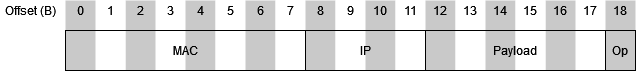
\includegraphics[width=\textwidth]{Images/main_message_format.png}
    \caption{Message format expected on the main manager interface.}
    \label{fig:main_message_format}
\end{figure}
\subsection{DSM Establishment}\label{subsection:DSM_establishment}
The desire to establish a DSM with the manager is expressed with an opcode of zero. In this case the first four bytes of the payload are reserved for the size of the shared memory, while the remaining two are set to zero. The decision of how large the DSM has to be, should be made by the RTCR, where considerations like number of protected processes and size of the checkpoints of these processes influence the size required. The first action the manager undertakes is to select a port on which this new DSM is to be established. The chosen solution for this is to increment through the ephemeral ports starting at 1025, as 1024 is already in use. The maximum possible port would then be 65535. It is unlikely that such a high amount of RTCRs wish to establish a DSM, therefore wraparounds are deemed to be irrelevant. Afterwards, the manager allocates the memory and passes start address, size and the selected port to a new POSIX-thread named "Broker\_thread", which currently only sets up a server to receive checkpoints and store them to the allocated memory, simulating a DSM. The DSM by Weidinger could not be used, as it was implemented for Genode 15.02, necessitating large porting efforts to get it to function on the current Genode version. 

On the side of the RTCR, after receiving the port the manager wants it to connect to, a thread also called "Broker\_thread" is spawned, which sends the first checkpoint when it first connects to the broker of the manager. This message contains the offset of the checkpoint in the memory of RTCR within the first four bytes, the size of this checkpoint within the next two bytes and then the actual checkpoint. On receipt by the broker thread of the manager, this checkpoint is then written to the previously allocated memory at the specified offset. It has to be remarked that the current size of the buffer which the checkpoint is written to during network relay is set to 1024 bytes. This value needs to be modified according to the maximum size of a serialised checkpoint.

Meanwhile the main thread of the manager inserts the MAC, IP and address of the memory shared with the RTCR running on the ECU identified by the previous two parameters to a map it maintains. This map is necessary to be able to access the correct memory and store a checkpoint when notified by an instance of RTCR using the address and later iterate over when choosing an RTCR to migrate to by contacting the interfaces using the stored IP-addresses. The remaining value, the MAC, is used as the primary key.

The next step is for the RTCR to notify the CMS, that this checkpoint was sent to its memory by utilising the next functionality, described in the following section.
\subsection{Storing of Checkpoints}
An opcode of one in a message sent to the main manager interface means that a new checkpoint was just sent to the broker and written to memory. In this case the entire six bytes of payload are utilised: the first four bytes are for the offset of the checkpoint in the "shared" memory, whereas the last two bytes represent the size of the checkpoint. Together with the information of where the memory resides on the machine of the manager, which it retrieves from the previously mentioned map using the MAC as key, the checkpoint can then be read and sent to the network addressed storage. This process is accomplished by another POSIX-thread, so that the main thread of the manager can return to its server functionality as quickly as possible. The thread receives the necessary information to connect to the NAS, i.e. IP and port, and the previously mentioned values of offset, size, MAC-address and map as passing parameters. The combined process of connecting to the manager, establishing a pseudo DSM, and subsequently storing a checkpoint is further visualised in a sequence diagram in figure \ref{fig:dsm-and-store_sequence}.
\begin{figure}
    \centering
    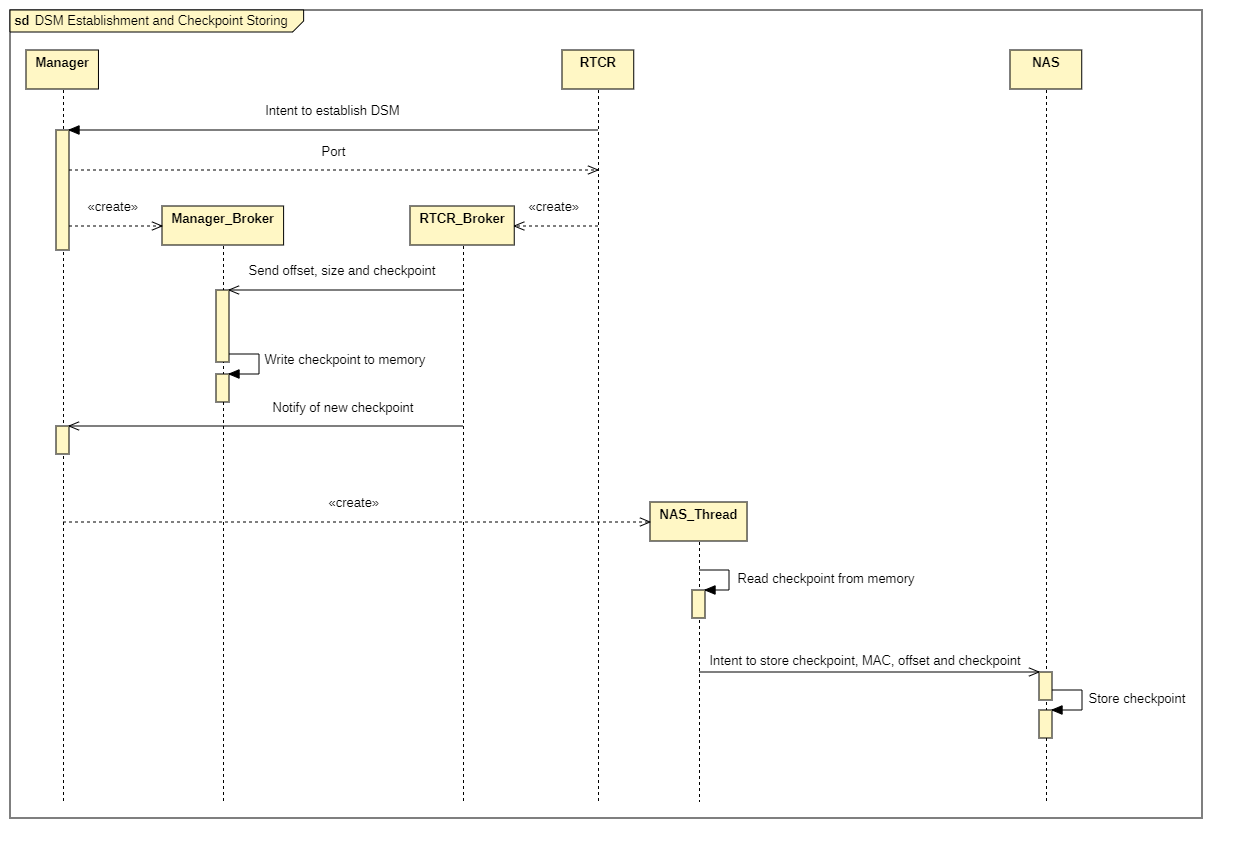
\includegraphics[width=1.25\textwidth, angle=90]{Images/dsm-and-store_sequence.png}
    \caption{Sequence diagram showing the establishment of a pseudo DSM and storing of a new checkpoint.}
    \label{fig:dsm-and-store_sequence}
\end{figure}
\subsection{Migration and Restoration}
A call for migration and restoration is stated by contacting the manager with an opcode of two. Hereby the payload of the message is used for the offset of the checkpoint, which together with the MAC address, uniquely identifies it. Resembling the interface for notification about a new checkpoint, the first four bytes are used for the offset, while in contrast to the aforementioned interface, the last two bytes remain unused. Another similarity is that a POSIX-thread is spawned to handle the actual process, again for the server to return to the beginning of its loop. This thread then performs the tasks of selecting a target to migrate to, retrieving the checkpoint from the NAS, and ultimately restoring it. The first task relies on an interface provided by the RTCR, as described in section \ref{section:Migration_and_Restoration}. However, no solution to the problem of determining CPU usage was found, resulting in only two parameters being prompted: available RAM and available capabilities. Both of these values are immediately sent to the client on connection to the socket always reachable on port 1025. Afterwards, the thread on the side of the manager creates a metric by multiplying the two parameters. As the available RAM is given in bytes, it is usually a much larger number than the remaining capabilities, making it the determinative parameter of the equation, but not as determinative as if the values where simply added. The behaviour of RAM being more important, but not so important, that an ECU with zero available capabilities could possible be selected for migration, is desired. The choice of metric in favour of multiplication was made due to this reason.

All to the manager known RTCRs, except the one calling for migration, are contacted by iterating over the map containing the MACs and IP-addresses, with the RTCR that returns the best combination of available RAM and capabilities being chosen for restoration. In the case of only one RTCR running in the system, the manager refuses the migration. This implementation is solely for testing and debugging purposes, as in the tested scenario of two RTCRs it is likely that when both RTCRs call for migration, one of them is chosen for both restorations. This is due to one RTCR always providing a better metric and both calls being performed simultaneously. This presents an issue in a real system, because at the time of an RTCR instance calling for migration for load balancing reasons, it has to terminate the process, or risk having a duplicate running on another system at the same time, if migration is successful. 

The logic described up to here is implemented by saving a tuple of two long integers, the first being the MAC address and the second being the metric for comparison of the currently deemed best ECU. During the iteration over the map, the metric calculation is skipped whenever the MAC at the current index and the MAC previously transmitted in the call for migration match. Otherwise, the information interface of the RTCR is contacted, the metric calculated, and then compared with the current best tuple, possibly setting a new one. How this is realised in code is presented in the following listing.
\begin{lstlisting}[language=C++, caption={Selection of suitable ECU for migration.}] 
Long_tuple best(0, 0);
for (int i = 0; i < map.size(); i++) {
    Genode::uint64_t current_mac = map.mac_at_index(i);
    if (mac == current_mac) continue;
    else {
        sockaddr.sin_addr.s_addr = htonl(map.ip_at(mac));
        if (connect(fd, (struct sockaddr *) &sockaddr, sizeof sockaddr) < 0) {
            Genode::error("[NAS thread -> migrate] Info socket connection failed");
            return nullptr;
        }
        Genode::uint64_t info_buf[2];
        recv(fd, info_buf, 2 * 8, 0);
        Genode::uint64_t metric = info_buf[0] * info_buf[1];
        if (metric >= best.get_second()) best.set(current_mac, metric);
    }
}
\end{lstlisting}
The next step is retrieving the checkpoint from the NAS. For this purpose the main NAS interface is contacted with the MAC and offset of the checkpoint desired to be restored. If this checkpoint can be found by the NAS, it is sent over the network back to the thread within the manager's domain. It then sends this checkpoint to a restoration interface on port 1026, where a symbolic restoration is performed by the RTCR dummy, i.e. printing its contents.
\section{Network Addressed Storage}
This section touches on the network addressed storage component (NAS) of the system scenario. In a real system, it would most likely consist of physical drives configured in RAID 1, accessible over network through a custom interface. The NAS component in this prototypical system represents just such an interface, with data being stored in its local memory without any failure safety. Not unlike the manager, the NAS acts as a server, discerning interface accesses by an opcode expected at a certain position. The message format is depicted in figure \ref{fig:NAS_message_format}. As previously mentioned in section \ref{subsection:DSM_establishment}, the message size of 1024 bytes is subject to change.
\begin{figure}
    \centering
    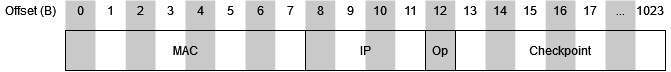
\includegraphics[width=\textwidth]{Images/NAS_message_format.png}
    \caption{Message format expected on the NAS interface.}
    \label{fig:NAS_message_format}
\end{figure}
There are two possible opcodes: An opcode of zero indicates that a checkpoint is being sent to the NAS for it to store, whereas an opcode of one means that a retrieval operation is to be performed. The NAS stores a checkpoint by first instantiating an object with the identifying parameters and the serialised checkpoint sent over Ethernet, now called "snapshot". Because the \verb|<std/vector>| library ported to Genode does not work with non-primitive data types such as the checkpoint object, a doubly linked list is implemented for checkpoint storage. Therefore, a checkpoint has a pointer to both the next and to the previous checkpoint in the list, while the main object of the NAS, in which execution is performed, has a pointer to the last checkpoint of the chain. The last checkpoint was chosen as the one to point to, because checkpoints are added at the end of the list. The class defining such a checkpoint is presented in the following code snippet. 
\newpage
\begin{lstlisting}[language=C++, caption={Checkpoint class used by the NAS.}] 
struct NAS::Checkpoint {
    Genode::uint64_t mac;
    Genode::uint32_t offset;
    Genode::uint8_t *snapshot;

    NAS::Checkpoint *previous;
    NAS::Checkpoint *next;

    Checkpoint(Genode::uint64_t mac, Genode::uint32_t offset, uint8_t *snapshot, NAS::Checkpoint *previous,
               NAS::Checkpoint *next) : mac(mac), offset(offset), snapshot(snapshot), previous(previous), next(next) {}

    ~Checkpoint() = default;
};
\end{lstlisting}
The act of storing a new checkpoint to memory ultimately consists of adding it to the linked list by modifying the necessary fields.
\newline \newline
Checkpoint retrieval is performed by iterating over the linked list by using a \verb|current| checkpoint pointer that, before entering the loop, is set to point to the last checkpoint in the list and at the end of the loop is set to its own predecessor. When the first object of the list, a null pointer, is reached, it is concluded that the checkpoint called for does not exist, upon which an exception is thrown. If the checkpoint could be found, it is sent to the client and removed from the list. The logic described up to this point can be seen in the following listing.
\newpage
\begin{lstlisting}[language=C++, caption={Checkpoint retrieval logic.}] 
auto current = reinterpret_cast<NAS::Checkpoint *>(last);
while (true) {
    if (current == nullptr) {
        Genode::error("Checkpoint for this MAC and offset could not be found");
        break;
    } else if (current->mac == mac && current->offset == offset) {
        Genode::log("Checkpoint retrieved, sending to manager");
        if (send(client, current->snapshot, 1024, 0) != 1024) {
            Genode::error("Message could not be sent");
            shutdown(fd, 0);
            return;
        }

        if (current->previous != nullptr) current->previous->next = current->next;
        if (current->next != nullptr) current->next->previous = current->previous;
        Genode::destroy(sliced_heap, current);
        break;
    }
    current = current->previous;
}
\end{lstlisting}